\documentclass[output=paper]{langsci/langscibook}
\ChapterDOI{10.5281/zenodo.1407011}
\selectlanguage{english}


\title{Troubles with flexemes}

\author{Anna M. Thornton\affiliation{University of L'Aquila}}

 \abstract{This paper investigates an aspect of the notion \emph{flexeme} (\ili{French} \emph{flexème}), introduced by %
%Fradin \& Kerleroux (2003)
\citet{Fradin03b}%
%Fradin-Kerleroux
%
, %
%Fradin (2003)
\citet{Fradin2003}%
%Fradin
%
. After a brief review of how this concept developed in these authors' work, and of how these authors conceive of lexemes\is{lexeme} (Section~\ref{what-are-flexemes}), the relation between flexemes and \isi{overabundance} %
%(Thornton 2011, 2012) 
\citep{Thornton11,Thornton12} %
%Thornton;Thornton
%
is explored. Overabundance\is{overabundance} is introduced in Section~\ref{overabundance}, and Section~\ref{non-canonical-mappings-between-lexemes-and-flexemes} is devoted to some case studies, from \ili{Italian} and other languages. It is shown that a single \isi{lexeme} can map to more than one flexeme -- and \isi{overabundance} results from this mapping. Besides, it is shown that flexemes differing from each other in parallel ways can have various relations with lexemes\is{lexeme}: in some cases, mapping to different flexemes distinguishes two lexemes\is{lexeme} that are homophonous in their citation form (e.g., \ili{Italian} \textsc{succedere}\textsuperscript{1} `happen' with \textsc{pst.ptcp}  \emph{successo} and \textsc{succedere}\textsuperscript{2} `succeed' with \textsc{pst.ptcp} \emph{succeduto}), while in other cases flexemes that differ from each other in a way parallel to the previous one map to a single overabundant\is{overabundance} \isi{lexeme} (e.g., \ili{Italian} \textsc{perdere} `lose' with \textsc{pst.ptcp} \emph{perso} and \emph{perduto}). I conclude that the distinction between lexemes\is{lexeme} and flexemes first proposed by %
%Fradin \& Kerleroux (2003)
\citet{Fradin03b} %
%Fradin-Kerleroux
%
 and %
%Fradin (2003)
\citet{Fradin2003}%
%Fradin
%
, as well as their definition of \isi{lexeme}, based on semantic and constructional coherence rather than on inflectional coherence, is useful even beyond the area of \isi{lexeme} formation for which it was originally proposed. }

\maketitle

\begin{document}
\selectlanguage{english}
\is{flexeme|(}



\section{Introduction}\label{introduction}

In a paper titled ``Troubles with lexemes\is{lexeme}'', Bernard Fradin and
Françoise Kerle\-roux %
% (2003) 
(\citeyear{Fradin03b}) %
%Kerleroux
%
laid the bases for a critique of the commonly
held notion of \isi{lexeme}, drawing data from the realm of word-formation.
They observed at the beginning of their paper:

\begin{quote}
the \isi{lexeme} is supposed to constitute one lexical unit. \textbf{This
unicity is guaranteed by inflection on the one hand} and by the semantic
content of the \isi{lexeme}, which is supposed to be unique, on the other
%
%(Fradin \& Kerleroux 2003: 177, emphasis mine)
\citep[177, emphasis mine]{Fradin03b}%
%Fradin-Kerleroux
%
.
\end{quote}

They proceeded then to show that the objects to which word-formation
rules apply -- which they propose to call lexemes\is{lexeme}, partially modifying
the usual definition of this term -- are semantically fully specified
objects, that are, however, unspecified for inflection. In the
concluding section of that paper, they propose to distinguish three
different theoretical entities: lexemes\is{lexeme} %
%(``lexical individuals defined
%by the conjunction of three properties: category, underspecification for
%inflection, full specification for meaning'', Fradin \& Kerleroux 2003:193)
\citep[``lexical individuals defined by the conjunction of three properties: category, underspecification for inflection, full specification for meaning'', ][193]{Fradin03b}%
%Fradin-Kerleroux
%
, syntactic words (which are inflected, categorized, and fully
specified for meaning), and a third entity, which they propose to call
\emph{inflecteme}\is{inflecteme|see {flexeme}} in \ili{English} and \emph{flexème}\is{flexeme} in \ili{French} %
%(see also
%Fradin 2003: 259)
\citep[see also ][259]{Fradin2003}%
%Fradin
%
. Objects of this third type are categorized,
uninflected and underspecified for meaning.

In this short contribution, I will discuss some aspects of these
entities that have come to the fore of the debate in morphology after
the publication of %
%Fradin \& Kerleroux (2003) 
\citet{Fradin03b} %
%Fradin-Kerleroux
%
and %
%Fradin (2003)
\citet{Fradin2003}%
%Fradin
%
. I
prefer to refer to these units as \emph{flexèmes}\is{flexeme}, because I think that
the intentional and witty phonological and orthographic overlap with
\emph{lexème} `\isi{lexeme}' is too good to be lost, and as an \emph{hommage}
to the authors who first proposed this term. Following %
%Fradin (to appear)
\citet{Fradin17}%
, in this paper I will use the \ili{English} adaptation \emph{flexeme}.

The paper is organized as follows: Section~\ref{what-are-flexemes} reviews the development of
the concept of flexeme; Section~\ref{overabundance} introduces the concept of
\isi{overabundance} in inflectional paradigms\is{paradigm}; Section~\ref{non-canonical-mappings-between-lexemes-and-flexemes} presents several case
studies from \ili{Italian} and other languages, illustrating cases in which a
single \isi{lexeme} is overabundant\is{overabundance} in one or more cells, i.e., maps to two
distinct flexemes; Section~\ref{conclusions} concludes.

\section{What are flexemes?}\label{what-are-flexemes}

In different contributions by Bernard Fradin, sometimes in collaboration
with Françoise Kerleroux, the concept of \emph{flexème}\is{flexeme}\slash{}flexeme is
presented differently: its coverage seems to have grown with time,
probably in consequence of our growing understanding of the workings of
inflectional morphology in the early years of the third millennium.

In %
%Fradin \& Kerleroux (2003: 193) 
\citet[193]{Fradin03b} %
%Fradin-Kerleroux
%
the concept seems to be equivalent to
that of \emph{stem}\is{stem} %
%(in the sense, e.g., of Aronoff 1994)
\citep[in the sense, e.g., of ][]{Aronoff94}%
%Aronoff
%
:

\begin{quote}
This unit {[}i.e., the \isi{inflecteme}\slash{}\emph{flexème}\is{flexeme}{]} lacks semantic
specification since it functions as the ``inflectional \isi{stem}''.
\end{quote}

However, the authors seem to have something more than just a single \isi{stem}
in mind, since immediately after this definition they observe: ``This is
correlated to the fact that ``no semantic constraints hangs {[}sic{]}
over the application of inflectional rules'' %
%(Corbin 1987: 6)
\citep[6]{Corbin87}%
%Corbin
%
''. So the
idea that flexemes have to do with instructions for building all the
inflected forms that realize a \isi{lexeme} seems to have been present already
in %
%Fradin \& Kerleroux (2003)
\citet{Fradin03b}%
%Fradin-Kerleroux
%
.

%
%Fradin (2003: 259) 
\citet[259]{Fradin2003} %
%Fradin
%
states that

\begin{quote}
Les flexèmes\is{flexeme} {[}\ldots{}{]} comportent {[}\ldots{}{]} des informations
relevant {[}\ldots{]} du syntactique interne (les différents thèmes
flexionnels, sous forme hiérarchisée, s'il en existe plusieurs
{[}\ldots{}{]}).
\end{quote}

So the concept of flexeme seems to have developed from being used to
refer to a \isi{stem} to being used to refer to the whole \isi{stem}-set\is{stem!stem-set} of a
\isi{lexeme}. In %
%Fradin (to appear)
\citet{Fradin17} %
 a new development appears.\footnote{The
  notion of flexeme is not mentioned in %
%Fradin \& Kerleroux (2009)
\citet{Fradin09}%
%Fradin-Kerleroux
%
.} The
author, dealing with verbs, distinguishes between verbs as morphological
units, called ``morphological verbs'', and verbs as lexical units,
called ``verbal lexemes\is{lexeme}''. He states that ``[m]orphologically, a V is
defined by its inflectional \isi{paradigm}'', and maintains that the two
\ili{French} verbs \textsc{ressortir\textsuperscript{1}} ((de Y): \emph{il
ressort, il ressortait}\ldots{}) `go out again' and
\textsc{ressortir\textsuperscript{2}} ((à Y): \emph{il ressortit, il
ressortissait\ldots{}}) `come under'``constitute distinct `flexemes',
see %
%Fradin \& Kerleroux (2003) 
\citet{Fradin03b} %
%Fradin-Kerleroux
%
{[}\ldots{}{]} because the set of their
word-forms is not identical'' %
%(Fradin to appear: 4)
\citep[4]{Fradin17}%
.

In this passage, Fradin attributes to \citet{Fradin03b}
a fully
developed concept of flexeme, in which a flexeme contains all the
information needed to generate all the inflectional forms in a \isi{paradigm}:
not only the information about which \isi{stem} to select, but also
inflectional class and realization rules for the different inflected
forms. Roughly, it seems to me, a flexeme now corresponds to the
entities called \emph{form paradigm}\is{paradigm!form paradigm} and \emph{realized paradigm}\is{paradigm!realized paradigm} in
paradigm-linkage theory\is{paradigm!paradigm-linkage theory} %
%(Stump 2016)
\citep{Stump16}%
%Stump
%
. %
%Fradin (to appear)
\citet{Fradin17} %
%
 also equates
the notion of flexeme with that of \isi{Paradigm Identifier} adopted by
%
%Bonami \& Tribout (2012)
\citet{Bonami12t}%
%Bonami-Tribout
%
. In turn, %
%Bonami \& Tribout (2012)
\citet{Bonami12t} %
%Bonami-Tribout
%
 state that
their notion of \isi{Paradigm Identifier} ``{[}c{]}aptures 
%Fradin and
%
%Kerleroux (2003)
\citet{Fradin03b}%
%Kerleroux
%
's notion of a flexeme: a family of lexemes\is{lexeme} with the
same inflectional \isi{paradigm}'' %
(%
%Bonami \& Tribout 2012
\citealt{Bonami12t}%
%
: slide 16).\footnote{The notion of \isi{Paradigm Identifier} is clearly articulated  by Bonami \& Crysmann (this volume).}
%\citep[slide 16.\footnote{The notion of Paradigm Identifier is clearly articulated   by Bonami \& Crysmann (this volume).}]{Bonami12t}%
%Bonami-Tribout
%


Papers such as %
%Fradin (to appear) 
\citet{Fradin17} %
%
%
and %
%Bonami \& Tribout (2012) 
\citet{Bonami12t} %
%Bonami-Tribout
%
address
the question of how to deal with objects that are semantically different
but morphologically identical, such as
\textsc{cirage\textsuperscript{1}} `polishing' and
\textsc{cirage\textsuperscript{2}} `shoe polish', or
\textsc{perler\textsuperscript{1}} `sew beads on' and
\textsc{perler\textsuperscript{2}} `form beads on', which share a
flexeme (a form paradigm\is{paradigm!form paradigm} and a realized paradigm\is{paradigm!realized paradigm}) but are different
lexemes\is{lexeme}.\footnote{This phenomenon is labelled ``homomorphy'' by %
%Stump  (2016: 65)
\citet[65]{Stump16}%
%
: ``homomorphic lexemes\is{lexeme} are lexically and semantically
  distinct but alike in every detail of their morphology''. \ili{English}
  examples are \textsc{wear\textsuperscript{1}} `have on (an article of
  clothing)' and \textsc{wear\textsuperscript{2}} `erode'.}

In this paper, on the contrary, I will explore the issue of objects that
are the same \isi{lexeme}, in the sense of %
%Fradin \& Kerleroux (2003) 
\citet{Fradin03b} %
%Fradin-Kerleroux
%
and
%
%Fradin (2003, to appear)
\citet{Fradin2003,Fradin17}%
%Fradin
%
, but can be realized, to variable degrees, by
different flexemes.

\section{Overabundance}\label{overabundance}
\largerpage
In recent years, attention has been drawn to the phenomenon of
\isi{overabundance} in inflectional paradigms\is{paradigm} %
%(Thornton 2011, Stump 2016:
%147-151)
\citep[147-151]{Thornton11,Stump16}%
%Thornton;Stump
%
. Overabundance\is{overabundance} is defined as the situation in which two or more
forms are available to realize the same cell in an inflectional
\isi{paradigm}; in terms of paradigm linkage theory\is{paradigm!paradigm-linkage theory}, one content cell has more
than one realization. %
%(Stump 2016: 148)
\citet[148]{Stump16} %
%Stump
%
gives an
example from \ili{English}. Consider the verbs \textsc{seem}, \textsc{mean},
and \textsc{dream}, and the realizations of their past tense:
$\langle$\textsc{seem}, \{past\}$\rangle$ is realized by \emph{seemed}, $\langle$\textsc{mean},
\{past\}$\rangle$ is realized by \emph{meant}, and $\langle$\textsc{dream}, \{past\}$\rangle$
can be realized either by \emph{dreamed} or by \emph{dreamt}. The two
(or more) forms that realize the same cell are sometimes called cell
mates %
%(Thornton 2011)
\citep{Thornton11}%
%Thornton
%
.

How does \isi{overabundance} relate to the notion of flexemes? Does the
existence of distinct but synonymous realizations for a given content
cell force us to recognize distinct flexemes linked to a single \isi{lexeme}?

%Fradin (to appear)
\citet{Fradin17} %
%
 analyzes cases such as
\textsc{perler\textsuperscript{1}} `sew beads on' and
\textsc{perler\textsuperscript{2}} `form beads on' as distinct lexemes\is{lexeme}
linked to the same flexeme. The case of \emph{dreamed}
`dream.\textsc{pst'} and \emph{dreamt} `dream.\textsc{pst'} appears to
be a mirror image of this case, with distinct flexemes linked to a
single \isi{lexeme}. The existence of such a state of affairs would be
predicted in Fradin's theory, in which lexemes\is{lexeme}, defined as categorized
and semantically fully specified but uninflected objects, are autonomous
from the flexemes that provide instructions for the realization of their
inflected forms. Recognizing the possibility that a single \isi{lexeme} may be
linked to two (or more) flexemes implies that a difference in
inflectional realization cannot be invoked as one of the criteria that
allow to distinguish between different lexemes\is{lexeme} vs. simply different
senses\slash{}acceptations of a polysemous \isi{lexeme}, as was sometimes done in
traditional discussions of the \isi{homonymy}\slash{}\isi{polysemy} distinction %
%(e.g.,
%Ullmann 1957: 127-132)
\citep[see e.g.][127--132]{Ullmann1957}%
%Ullmann
%
.\footnote{Remember also the observation by %
%Fradin
%  \& Kerleroux (2003: 177) 
\citet[177]{Fradin03b} %
%Fradin-Kerleroux
%
quoted in Section~\ref{introduction}, that unicity of a \isi{lexeme} ``is
  guaranteed by inflection'' as well as by the semantic content.}
Indeed, flexemes that are distinct in parallel ways may map to a single
\isi{lexeme} or to distinct lexemes\is{lexeme} -- where the criterion for recognizing
distinct lexemes\is{lexeme} is semantic and constructional difference, as proposed
by %
%Fradin \& Kerleroux (2003, 2009) 
\citet{Fradin03b,Fradin09} %
%Fradin-Kerleroux;Fradin-Kerleroux
%
and %
%Fradin (2003, to appear)
\citet{Fradin2003,Fradin17}%
%Fradin
%
.

In the following section, I will review some data that show that the
mapping between flexemes and lexemes\is{lexeme} can be of several kinds.

\section{Non-canonical mappings between lexemes\is{lexeme} and
flexemes}\label{non-canonical-mappings-between-lexemes-and-flexemes}

In this section, I will present data, mostly from well-studied cases in
familiar languages, that show how one and the same difference in
inflectional realization may map either to distinct lexemes\is{lexeme} or to a
single overabundant\is{overabundance} \isi{lexeme}.

\subsection{Case study 1: Noun plurals}\label{case-study-1-noun-plurals}
\is{noun!plural|(}

Nouns in which apparently more than one plural form pairs with a single
singular form are very easy to find in language descriptions. Usually
authors assume, at least implicitly, the admittedly vaguely defined
criterion of `difference in meaning' to decide whether specific cases
represent distinct lexical items with homophonous singular forms or a
single lexical item which is overabundant\is{overabundance} in its plural cell(s).
Besides, since data are usually found in works which aim at description
rather than at theoretical analysis, often authors leave the matter
undecided, because it is not necessary for descriptive purposes to
establish whether a certain case is an instance of \isi{homonymy} or \isi{polysemy};
on the other hand, cases in which no semantic distinction is observable
between two or more different plural forms are usually highlighted by
authors of descriptions.

\newpage
Cases such as the \ili{English} and \ili{Breton} ones in (\ref{ex:Thornton:1}) and (\ref{ex:Thornton:2}) are typical:

\ea\label{ex:Thornton:1} \ili{English} %
%(Aronoff 2000: 347)
\citep[347]{Aronoff2000b}%
%Aronoff
%


\ea\label{ex:Thornton:1a}{\textsc{sg} \emph{brother} \textsc{pl} \emph{brothers}}\\
\glt `male sibling' \\

\ex\label{ex:Thornton:1b} \textsc{sg} \emph{brother} \textsc{pl} \emph{brethren}\\
\glt `fellow member of a profession, society or sect' \\

\z

\ex \label{ex:Thornton:2} \ili{Breton} %
%(Trépos 1980) 
\citep{Trepos1980} % 1980 première édition citée par Anna, changée à 1994
%?Trépos
%
\footnote{\ili{Breton} nouns inflect only for number.}


\ea \label{ex:Thornton:2a}\textsc{sg} \emph{eskob} \textsc{pl} \emph{eskibien}\\
\glt `bishop'\\


\ex \label{ex:Thornton:2b}\textsc{sg} \emph{eskob} \textsc{pl} \emph{eskobou}\\
\glt `kingpin'\footnote{The French gloss given by %
%Trépos (1980:73) 
\citet[73]{Trepos1980} %
%?Trépos
%
for
  \emph{eskibien} is `chevilles d'attelage'.}\\
\z
\z

In these cases most authors argue that the meanings of the two items are
sufficiently distinct to allow us to consider them as distinct lexemes\is{lexeme},
which happen to be homophon\-ous in their singular form.\footnote{Even if
  (\ref{ex:Thornton:1b}) obviously derives from (\ref{ex:Thornton:1a}) by means of a metaphorical extension.}
In these cases, then, we have a 1:1 mapping between lexemes\is{lexeme} and
flexemes, with the extra quirk represented by the fact that two distinct
flexemes have homophonous singular forms.

However, by perusing the whole description of \ili{Breton} noun plural offered
by %
%Trépos (1980)
\citet{Trepos1980}%
%?Trépos
%
, we discover that `bishop' can have as many as three
different plural forms (\ref{ex:Thornton:3a}), and the same is true for `coat' (\ref{ex:Thornton:3b}):

\ea\label{ex:Thornton:3} \ili{Breton} %
%(Trépos 1980: § 149)
\citep[§ 149]{Trepos1980}%
%?Trépos
%


\ea\label{ex:Thornton:3a}\textsc{sg} \emph{eskob} \textsc{pl} \emph{eskibien\slash{}eskobed /
eskeb}\\
\glt `bishop'\\

\ex\label{ex:Thornton:3b}\textsc{sg} \emph{mantell} \textsc{pl} \emph{mentell\slash{}mentellou\slash{}mentilli}\\
\glt `coat'\\
\z
\z

A similar situation is common in Modern Standard Arabic\il{Arabic!Modern Standard}, where nouns
often have several plural forms; authors of descriptions usually comment
on when they would prefer to assign the different plural forms to
distinct lexemes\is{lexeme}, on the basis of a clear distinction in meaning, as in
(\ref{ex:Thornton:4a} vs. \ref{ex:Thornton:4b}, \ref{ex:Thornton:4c} vs. \ref{ex:Thornton:4d}), and when the different plural forms can be used
interchangeably, and must be recognized as realizing the same \isi{lexeme}, as
in (\ref{ex:Thornton:5a}-\ref{ex:Thornton:5b}).

\newpage 
\ea\label{ex:Thornton:4} Modern Standard Arabic\il{Arabic!Modern Standard} %
%(Holes 2004, Kaye 2007)
\citep{Holes2004,Kaye2007}% Holes 2004 dans l'original => 1995 dans la biblio
%?Holes;Kaye
%
\footnote{MS Arabic\il{Arabic!Modern Standard}
  nouns inflect for number (singular, dual, plural), case (nominative,
  genitive, accusative, with a syncretism of genitive and accusative
  (sometimes called oblique) in non-singular forms), and definiteness
  (definite, indefinite). In systems in which nouns inflect for other
  features besides number, if multiple forms with the same number value
  exist they are predicted to exist in all cells; e.g., in \ili{Arabic},
  multiple plural forms are predicted to exist in all case and
  definiteness values.}

\ea\label{ex:Thornton:4a}\textsc{sg} \emph{bayt} \textsc{pl} \emph{buyu:t}\\
\glt  `tent', `house'\glt

\ex\label{ex:Thornton:4b}\textsc{sg} \emph{bayt} \textsc{pl} \emph{ʔabya:t}\\
\glt  `verse of poetry'\\

\ex\label{ex:Thornton:4c}\textsc{sg} \emph{maktab} \textsc{pl} \emph{maka:tib}\\
\glt  `office'\\

\ex\label{ex:Thornton:4d}\textsc{sg} \emph{maktab} \textsc{pl} \emph{maktaba:t}\\
\glt  `library', bookshop'
\z

\ex\label{ex:Thornton:5} Modern Standard Arabic\il{Arabic!Modern Standard} %
%(Kaye 2007)
\citep{Kaye2007}%
%Kaye
%


\ea\label{ex:Thornton:5a}\textsc{sg} \emph{ʕayn} \textsc{pl} \emph{ʔaʕyun\slash{}ʕuyūn}\\
\glt `eye'\\


\ex\label{ex:Thornton:5b}\textsc{sg} \emph{sāriq} \textsc{pl} \emph{sāriqūn, saraqa, surrāq}\\
\glt `thief' \\
\z
\z

With respect to nouns such as those in (\ref{ex:Thornton:5}), \citet[234--235]{Kaye2007} 
observes that ``[t]here are many nouns with two or more plural variants
without any difference in meaning'', while on the nouns in (\ref{ex:Thornton:4a}-\ref{ex:Thornton:4b}) he
states that ``[i]t is best to regard {[}\ldots{}{]} \emph{bayt} as
distinct lexemes\is{lexeme}'' %
%(Kaye 2007: 234)
\citep[234]{Kaye2007}%
%Kaye
%
.

Authors like Kaye rely on meaning distinction as the only criterion for
distinguishing between lexemes\is{lexeme}, and (implicitly) accept the possibility
that what they conceive of as single lexemes\is{lexeme} (like the ones in (\ref{ex:Thornton:5})) may
have overabundant\is{overabundance} realizations in one or more cells, i.e., may map to
more than one flexeme. Other authors, however, reject this possibility,
and assume that a difference in inflectional realization (a difference
in flexemes) must always correspond to a difference in lexemes\is{lexeme}. A
champion of such a position is Paolo Acquaviva, who has articulated his
point of view in his work on \ili{Italian} double noun plurals %
%(Acquaviva 2008)
\citep{Acquaviva2008}%
%Acquaviva
%
.

\ili{Italian} nouns have inherent gender\is{gender} (with two values: feminine and
masculine) and inflect for number (with two values: singular and
plural). About 20 \ili{Italian} nouns are usually described as overabundant\is{overabundance} in
the plural (e.g., in traditional reference grammars such as %
%Battaglia \& Pernicone 1954
\citealt{BattagliaPernicone1954}%
%
). These nouns have a singular form in \emph{-o} which is
masculine, a plural form in \emph{-i} which is masculine, and a plural
form in -\emph{a} which is feminine. Some representative examples are
given in (\ref{ex:Thornton:6}):

\ea\label{ex:Thornton:6} \ili{Italian} %
%(Acquaviva 2008, Thornton 2010-2011{[}2013{]})
\citep{Acquaviva2008,Thornton2011b}%
%Acquaviva;Thornton
%


\ea\label{ex:Thornton:6a}\textsc{sg} \emph{braccio} \textsc{pl} \emph{braccia}\slash{}\emph{bracci}\\
\glt `arm'\\

\ex\label{ex:Thornton:6b}\textsc{sg} \emph{corno} \textsc{pl} \emph{corna}\slash{}\emph{corni}\\
\glt `horn'\\

\ex\label{ex:Thornton:6c}\textsc{sg} \emph{ginocchio} \textsc{pl} \emph{ginocchia}\slash{}\emph{ginocchi} \\ \glt`knee'\\

\ex\label{ex:Thornton:6d}\textsc{sg} \emph{membro} \textsc{pl} \emph{membra}\slash{}\emph{membri}\\
\glt`limb'\slash{}`member'\\
\z
\z

Acquaviva's position is that plurals in -\emph{a}, independently of
whether they differ in meaning from the plurals in \emph{-i} with which
they share a root, are distinct lexemes\is{lexeme}, \emph{pluralia tantum}\is{noun!\emph{pluralia tantum}},
derivationally related to the lexemes\is{lexeme} in \emph{-o\slash{}-i} with which they
share a root:

\begin{quote}
plurals in -\emph{a} {[}\ldots{}{]} are lexical plurals:
\textbf{distinct, inherently plural nouns}, related to the base noun by
a word-formation process. %
%(Acquaviva 2008: 123, emphasis mine)
\citep[123, emphasis mine]{Acquaviva2008}%
%Acquaviva
%


\textbf{\emph{Braccia} `arms' is not the plural of \emph{braccio}
`arm'}; it is an inherently plural \isi{lexeme}, derived from the same root as
\emph{braccio\slash{}bracci} %
%(Acquaviva 2008: 157, emphasis mine)
\citep[157, emphasis mine]{Acquaviva2008}%
%Acquaviva
%
\end{quote}

He brings forward several arguments for his position, which are reviewed
in %
%Thornton (2010-2011{[}2013{]}: 430-438)
\citet[430--438]{Thornton2011b}%
%Thornton
%
, where it is shown that one
of them (agreement with conjoined singular NPs) is based on a
misunderstanding of the workings of \ili{Italian} agreement resolution rules,
and can be dismissed as irrelevant. His other arguments will be
illustrated here.

The first argument is purely metatheoretical. Acquaviva states it as
follows:

\begin{quote}

The simple fact that a number of plurals in \emph{-a} do not block their
regular alternants in -\emph{i} is enough to prove the point, \textbf{if
we take seriously inflectional disjunctivity} %
%(Acquaviva 2008: 145,
%emphasis mine)
\citep[145, emphasis mine]{Acquaviva2008}%
%Acquaviva
%
.
\end{quote}

This argument boils down to positing as a theoretical requirement the
non-existence of \isi{overabundance}, or the impossibility of a single \isi{lexeme}
to map to distinct flexemes. Such a choice eliminates the problem we are
investigating by denying its existence, rather than by offering a
solution. However, if we assume, as done in the canonical approach to
morphological typology %
%(Corbett 2005, 2006, 2007)
\citep{Corbett2005,Corbett2006,Corbett2007}%
%Corbett;Corbett;Corbett
%
, that inflectional
disjunctivity and lack of \isi{overabundance} are only canonical properties of
lexemes\is{lexeme}, rather than inviolable theoretical requirements, the problem
reappears and requires to be investigated.

Another argument put forward by Acquaviva to establish that plurals in
-\emph{a} are distinct lexemes\is{lexeme} from their co-radicals in -\emph{o\slash{}-i} is
consonant with 
Fradin \& Kerle\-roux's~(\citeyear{Fradin03b}) view of lexemes\is{lexeme}: Acquaviva
observes that some plurals in -\emph{a} appear to be the bases of
word-formation processes. An example would be \emph{cornificare} `to
make a cuckold of', which Acquaviva analyzes as derived from
\emph{corna} `horns' (\ref{ex:Thornton:6b}); \emph{cornificare} is synonymous with the
idiom \emph{fare\slash{}mettere le corna} `to make a cuckold of, lit. to make
\slash{}put horns.\textsc{f.pl}', which is never realized by
*\emph{fare\slash{}mettere i corni,} with `horns.\textsc{m.pl}'. On this basis,
one can presume that \emph{corna}, and not \emph{corni}, is the base of
\emph{cornificare}. However, the idiom \emph{fare\slash{}mettere un corno}
`to make a cuckold of, lit. to make\slash{}put a horn.\textsc{m.sg}' is also
attested, so one cannot exclude that the base of \emph{cornificare} is a
non-\isi{defective} \isi{lexeme} \emph{corno\slash{}corna}, rather than a \emph{plurale
tantum}\is{noun!\emph{pluralia tantum}} \isi{defective} noun \emph{corna}. In any case, this argument boils
down to recognizing different lexemes\is{lexeme} when there is a difference in
semantics and in the possibility of appearing in certain constructions,
as proposed also by %
%Fradin \& Kerleroux (2003, 2009)
\citet{Fradin03b,Fradin09}%
%Fradin-Kerleroux;Fradin-Kerleroux
%
, %
%Fradin (2003)
\citet{Fradin2003}%
%Fradin
%
.
This is orthogonal to the question whether a \isi{lexeme}, defined on the
basis of its semantics and distribution in constructions, can be
overabundant\is{overabundance} in one or more cells. If we show that two plural forms
appear in the same set of environments and constructions, they must be
recognized as belonging to the same \isi{lexeme} (unless, like Acquaviva, one
wants to posit a difference of inflectional realization as sufficient
for recognizing distinct lexemes\is{lexeme}, regardless of the equal semantics and
distribution of the forms). %
%Thornton (2010-2011{[}2013{]}) 
\citeauthor{Thornton2011b}~(2010-2011) 
has shown, by
means of corpus-based evidence, that in some cases two plurals in
-\emph{i} and -\emph{a} are used interchangeably in the same context,
and cannot therefore be considered as instances of distinct lexemes\is{lexeme} in
%
%Fradin \& Kerleroux (2003)
\citet{Fradin03b}%
%Fradin-Kerleroux
%
's sense. This is the case for \emph{ginocchi
\slash{}ginocchia} `knees' (\ref{ex:Thornton:6c}), both of which appear interchangeably (as well
as the singular form \emph{ginocchio}) in a number of syntactic
environments 
(\citealt{Thornton2011b}: 465). In the case of
\emph{membra} and \emph{membri} (\ref{ex:Thornton:6d}), instead, there is evidence to
posit two distinct lexemes\is{lexeme}, \textsc{membro\textsuperscript{1}} `limb
(body part)', which is {[}$-$human{]}, and
\textsc{membro\textsuperscript{2}} `member (of a committee,
organization, etc.)', which is {[}+human{]}, and is obviously derived
from \textsc{membro\textsuperscript{1 }}by means of a metaphoric
extension. \textsc{membro\textsuperscript{2 }}is not overabundant\is{overabundance}: its
plural is always \emph{membri}, and it is the base of a derived feminine
\textsc{membra} `female member (of a committee, organization, etc.)',
\textsc{pl} \emph{membre} %
%(Thornton 2014)
\citep{Thornton2014}%
%Thornton
%
.
\textsc{membro\textsuperscript{1 }}isn't overabundant\is{overabundance} either: its plural
is \emph{membra} `limbs'; however, contrary to Acquaviva's analysis, it
is not \isi{defective}: the singular \emph{membro} in the sense of `limb, body
part' is attested 
(cf. \citealt{Thornton2011b}: 463, fn.~38). These
examples show that each case in which we observe, in \ili{Italian}, a feminine
plural in -\emph{a} and a masculine one in -\emph{i} based on the same
root, must be analyzed in its own right: the parallelism in the flexemes
does not guarantee a parallelism in the lexemes\is{lexeme}. \emph{Membri} and
\emph{membra} belong to different lexemes\is{lexeme} (defined according to %
%Fradin
%\& Kerleroux's (2003) 
\citepos{Fradin03b} %
%Fradin-Kerleroux
%
and %
%Fradin's (2003) 
\citepos{Fradin2003} %
%Fradin
%
semantic criteria), while
\emph{ginocchi} and \emph{ginocchia} belong to the same \isi{lexeme} -- if we
admit the possibility of \isi{overabundance}, i.e. of a single \isi{lexeme} mapping
to more than one flexeme. The case of \emph{bracci} and \emph{braccia}
is particularly complex: these very frequent forms, if submitted to
%
%Fradin \& Kerleroux's (2003) 
\citepos{Fradin03b} %
%Fradin-Kerleroux
%
and %
%Fradin's (2003) 
\citepos{Fradin2003} %
%Fradin
%
criteria for the
recognition of distinct lexemes\is{lexeme}, map to several semantically distinct
lexemes\is{lexeme}, some of which are overabundant\is{overabundance} in the plural (e.g., `arm (body
part)'), while others select only one plural form (e.g., `ell (measure
of length)' selects \emph{braccia}). Again, the mapping between lexemes\is{lexeme}
and flexemes is not 1:1, as shown in Figure \ref{fig:Thornton:1}.

\begin{figure}
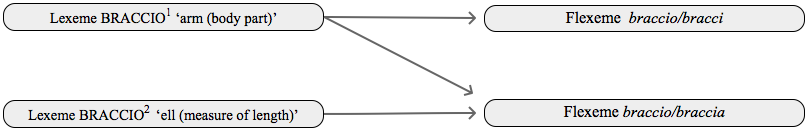
\includegraphics[width=1\textwidth]{figures/ThorntonFig1.png}
\caption{Mapping between two lexemes\is{lexeme} and two flexemes in \ili{Italian}}
\label{fig:Thornton:1}
\end{figure}
\is{noun!plural|)}

\subsection{Case study 2: Past
participles}\label{case-study-2-past-participles}
\is{verb!past participle|(}

Another area in which mapping between semantically defined lexemes\is{lexeme} and
flexemes is not always 1:1, and in which differences in flexemes do not
invariably coincide with differences in lexemes\is{lexeme}, is verbal inflection.

In some cases, two semantically and constructionally distinct lexemes\is{lexeme}
have quite different realized paradigms\is{paradigm!realized paradigm}, even if the citation forms
coincide. A case in point is that of \ili{Italian}
\textsc{succedere\textsuperscript{1}} `happen' and
\textsc{succedere\textsuperscript{2}} `succeed'.
\textsc{succedere\textsuperscript{1}} `happen' is an impersonal verb,
which is used only in 3\textsuperscript{rd} person forms; its
\textsc{pst.ptcp} is \emph{successo}.
\textsc{succedere\textsuperscript{2}} `succeed' is a bi-argumental verb;
its second argument is introduced by the preposition \emph{a} `to'; it
has a full set of realized forms, and its \textsc{pst.ptcp} is
overabundant\is{overabundance}, according to various authoritative sources %
%(Zingarelli
%2016, Serianni 1988)
\citep{Zingarelli2016,Serianni1988}%
%Serianni
%
: it can be either \emph{succeduto} or
\emph{successo}. The forms are shown in (\ref{ex:Thornton:7}):


\ea\label{ex:Thornton:7} \ili{Italian} %
(%
%Zingarelli 2016, Serianni 1988
\citealt{Zingarelli2016,Serianni1988}%
%
, personal knowledge)
%\citep[Zingarelli 2016, ][, personal knowledge]{Serianni1988}%
%Serianni
%

\begin{tabular}{@{}ll}
lexeme & \textsc{pst.ptcp}\\
\textsc{succedere\textsuperscript{1}} `happen' &\emph{successo}\\
\textsc{succedere\textsuperscript{2}} `succeed' &\emph{successo\slash{}succeduto}\\
\end{tabular}
\z

From (\ref{ex:Thornton:7}) it would appear that \textsc{succedere\textsuperscript{1 }}maps
to a single flexeme, while \textsc{succedere\textsuperscript{2 }}\newline maps to
two. However, for \textsc{succedere\textsuperscript{2 }} the form
\emph{succeduto} is prescribed over \emph{successo} by normatively
oriented sources like %
%Serianni (1988: § 316)
\citet[§ 316]{Serianni1988}%
%Serianni
%
\emph{,} and the most recent
example of \emph{successo} as a form of
\textsc{succedere\textsuperscript{2 }}cited by %
%Serianni (1988) 
\citet{Serianni1988} %
%Serianni
%
is from a
novel published in 1960. Investigation of contemporary usage in corpora
is difficult for practical reasons: \emph{successo} has 87763 tokens in
the corpus \emph{la Repubblica 1985-2000} (380M tokens; I will consider data from this corpus as representative of contemporary \ili{Italian} usage of \emph{successo} and \emph{succeduto}), making it
impractical to examine each token to assign it to either
\textsc{succedere\textsuperscript{1 }}or
\textsc{succedere\textsuperscript{2}}. Besides, \emph{successo} is a
homonym of the \textsc{sg} form of the noun \textsc{successo} `success'.
However, manual examination of the first 200 random tokens of the string
\emph{successo a}, which corresponds to both `happened to' and
`succeeded to', suggests that in this context \emph{successo} always
realizes \textsc{succedere\textsuperscript{1}} `happen', while, as
expected, all the 374 tokens of \emph{succeduto} in the corpus \emph{la
Repubblica 1985-2000} realize \textsc{succedere\textsuperscript{2}}
`succeed'. So, as far as the \textsc{pst.ptcp} is concerned, it appears
that in contemporary \ili{Italian} the two lexemes\is{lexeme}
\textsc{succedere\textsuperscript{1}} `happen' and
\textsc{succedere\textsuperscript{2}} `succeed' map to different
flexemes.\footnote{Things are more complicated with the simple past,
  which is (exemplifying with \textsc{3sg} forms) \emph{successe} for
  \textsc{succedere\textsuperscript{1 }}and overabundant\is{overabundance} for
  \textsc{succedere\textsuperscript{2}} (\emph{successe}\slash{}  \emph{succedette;} a third form, \emph{succedé}, is theoretically
  possible as `succeed.\textsc{pst.3sg}', but it is not attested in the
  corpus \emph{la Repubblica 1985-2000}). \emph{Successe} has 1263
  tokens and \emph{succedette} 43 tokens in this corpus; all tokens of
  \emph{succedette} realize \textsc{succedere\textsuperscript{2}}
  `succeed'; manual examination of the 14 tokens of the string
  \emph{successe a} `happened to\slash{}succeeded to' reveals that in most
  cases it realizes \textsc{succedere\textsuperscript{1}} `happen', but
  in 2 cases \emph{successe} realizes
  \textsc{succedere\textsuperscript{2}} `succeed', confirming that this
  verb is overabundant\is{overabundance} in its simple past. However, the simple past does
  not belong to the native grammar of many speakers of \ili{Italian}, for whom
  it is a learned form; so it is unwise to draw strong conclusions from
  these data. Overabundance\is{overabundance} in the simple past in \ili{Italian} shall be left
  for further research.}

We can compare this situation with that of the verb \textsc{perdere}
`lose', which is genuinely overabundant\is{overabundance} in its \textsc{pst.ptcp}, as
shown in (\ref{ex:Thornton:8}):

\largerpage[-1]
\ea\label{ex:Thornton:8} \ili{Italian} (personal knowledge)

\begin{tabular}{@{}ll}
lexeme & \textsc{pst.ptcp}\\

\emph{perdere} `lose' & \emph{perso\slash{}perduto}\\
\end{tabular}
\z
Speakers appear unaware of conditions regulating the selection of either
one of the two forms, to the point that many speakers asked the
\emph{Accademia della Cru\-sca}'s linguistic consulting service for advice
on when to use each form %
%(Thornton 2016)
\citep{Thornton2016}%
%Thornton
%
. Speakers seem convinced that
rules that govern a \isi{complementary distribution} of the two forms should
exist, but indeed the distribution of the two \textsc{pst.ptcp} forms is
not complementary: they can be used interchangeably in many contexts,
including idioms, as shown in (9a-b) and already shown by %
%Thornton (2011: 369)
\citet[369]{Thornton11}%
%
; the only case in which only one form is used is in titles
of works of art (\ref{ex:Thornton:9c}). Representative data, with frequencies from the
corpus \emph{la Repubblica} \emph{1985-2000} when relevant, are
presented in (\ref{ex:Thornton:9}).

\ea\label{ex:Thornton:9} \ili{Italian} %
(%
%Thornton 2011
\citealt{Thornton11}%
%
: 369, 
%2016
\citealt{Thornton2016}%
%
, personal knowledge)
%\citep[369, 2016, personal knowledge]{Thornton11}%
%Thornton
%


\ea\label{ex:Thornton:9a}\emph{occasione perduta} 291 / \emph{occasione persa} 83\\ \glt `a chance lost'\\

\ex\label{ex:Thornton:9b}\emph{perso la guerra} 109 / \emph{perduto la guerra} 32\\ \glt `lost the war'\\

\ex\label{ex:Thornton:9c}\emph{I predatori dell'arca perduta\slash{}*persa}\\ \glt `Raiders of the lost ark'\\

\ex\emph{Alla ricerca del tempo perduto\slash{}*perso}\\
\glt \emph{À la recherche du
temps perdu} by Proust, literally `In search of lost time'; English translation's title `Remembrance of things past'

\ex\emph{Paradiso perduto\slash{}*perso}\\\glt `Paradise lost' \\

\z\z
This case study shows again a case in which similar differences in
flexemes do not map in a parallel way to differences in lexemes\is{lexeme}: while
\textsc{succedere\textsuperscript{1}} `happen' and
\textsc{succedere\textsuperscript{2}} `succeed' map to distinct
flexemes, in which the \textsc{pst.ptcp} forms are \emph{successo} and
\emph{succeduto} respectively, \textsc{perdere} `lose' maps to two
flexemes, distinct from each other in a way parallel to the flexemes
\textsc{succedere\textsuperscript{1}} and
\textsc{succedere\textsuperscript{2}}, and its \textsc{pst.ptcp} can be
realized by both \emph{perso} and \emph{perduto}.
\is{verb!past participle|)}

\subsection{Systematic \isi{overabundance}\is{overabundance!systematic} and \isi{overabundance} in all
cells}\label{systematic-overabundance-and-overabundance-in-all-cells}

The two case studies illustrated above have shown examples in which
there is an overabundant\is{overabundance} cell in the form paradigm\is{paradigm!form paradigm} and the realized
paradigm of certain lexemes\is{lexeme} (such as \ili{Italian}
\textsc{braccio\textsuperscript{1}} `arm' and \textsc{perdere} `lose').
Technically, this should be enough to recognize that such lexemes\is{lexeme} map to
distinct flexemes. However, if one wished to take into account
quantitative considerations, one might want to deal with these cases by
recognizing a minor ``exception'', and still posit a single flexeme with
a single exceptional, overabundant\is{overabundance} cell.


\largerpage[-1]
However, \isi{overabundance} is not always confined to a single cell. In this
section I will illustrate cases of ``systematic overabundance\is{overabundance!systematic}'' %
%(Bonami
%\& Stump 2016: 469)
\citep[469]{Bonami:Stump16:PFM}%
%Bonami-Stump
%
, in which entire slabs\is{slab} or subparadigms\is{paradigm!sub-paradigm} are
involved,\footnote{The notion of slab\is{slab} has been introduced by %
%Carstairs  (1987: 81)
\citet[81]{Carstairs1987}%
%
, who defines it as ``a subset of the macroinflexions within
  one \isi{paradigm} consisting of all the macroinflexions which are
  associated with some specified morphosyntactic property''. His
  examples from Latin noun paradigms\is{paradigm} are the singular slab\is{slab} (all singular
  case-forms) or the genitive slab\is{slab} (\textsc{gen.sg} and
  \textsc{gen.pl}). The notion of sub-paradigm\is{paradigm!sub-paradigm} is used in a variety of
  senses, most commonly by scholars with a background in Slavonic
  languages. It aims at capturing sub-sets of cells in a \isi{paradigm} which
  share more than just one feature value, such as verb tenses (the
  Present Indicative, the Present Subjunctive, etc.).} and cases of
\isi{overabundance} in all cells. These cases definitely deserve consideration
in the context of exploring the possible deviations from a 1:1 mapping
between lexemes\is{lexeme} and flexemes.

A particularly clear example of systematic overabundance\is{overabundance!systematic} is found in
\ili{Spanish}, where all verbs have two complete sets of forms, built by means
of different endings, in the Imperfect Subjunctive, as shown in Table \ref{tab:Thornton:1} for the verb \emph{haber} `have'.

  \begin{table}
  \begin{tabular}{lll}
  \lsptoprule
  & -\emph{ra} set  & -\emph{se} set\\
  \midrule
  \textsc{1sg\slash{}3sg} & \emph{hubiera} & \emph{hubiese}\\
  \textsc{2sg} & \emph{hubieras} & \emph{hubieses}\\
  \textsc{1pl} & \emph{hubiéramos} & \emph{hubiésemos}\\
  \textsc{2pl} & \emph{hubiérais} & \emph{hubiéseis}\\
  \textsc{3pl } & \emph{hubieran} & \emph{hubiesen}\\
  \lspbottomrule
  \end{tabular}
  \caption{Imperfect Subjunctive of \ili{Spanish} \textit{haber} `have'}
  \label{tab:Thornton:1}
  \end{table}

Despite a suggestion by %
%Bolinger (1956) 
\citet{Bolinger1956} %
%Bolinger
%
that there is some subtle
semantic difference between the two sets of forms, contemporary
descriptions agree that ``these two sets of forms are interchangeable''
%
%(Butt \& Benjamin 2000:167; see also Rojo \& Veiga (1999:2910)
(\citet[167]{ButtBenjamin2000}; see also \citet[2910]{RojoVeiga1999}: ``las
formas en -\emph{ra} y -\emph{se} son hoy por hoy perfectamente
equivalentes''). \ili{Spanish} verbal lexemes\is{lexeme}, then, appear to systematically
map to two flexemes, which are distinct in the Imperfect Subjunctive
forms -- unless one wants to build \isi{overabundance} within the definition
of \ili{Spanish} verbal flexemes, exactly because of its systematicity.

In other cases, however, we encounter \isi{overabundance} in all cells of a
given \isi{lexeme}, but this is not systematic across all the lexemes\is{lexeme} within
that part of speech in the language; therefore, the possibility of
building \isi{overabundance} in the definition of the flexemes to which these
lexemes\is{lexeme} map is not viable, and we must recognize a 1:2 mapping between
lexemes\is{lexeme} and flexemes.

A case in point is that of the \ili{Italian} noun \textsc{orecchio} `ear'.
This noun can be described as overabundant\is{overabundance} in all its cells: it has two
\textsc{sg} forms and two \textsc{pl} forms, as shown in (\ref{ex:Thornton:10}):

\ea\label{ex:Thornton:10} \ili{Italian} (personal knowledge)

\begin{tabular}{@{}lll}
lexeme & \textsc{orecchio} & \\
\textsc{sg} forms& \emph{orecchio} \textsc{(m)} &
\emph{orecchia} \textsc{(f)}\\

\textsc{pl} forms& \emph{orecchi} \textsc{(m)} &
\emph{orecchie} \textsc{(f)}\\
\end{tabular}
\z

Of course, one could posit two distinct lexemes\is{lexeme}, \textsc{orecchio(m)}
and \textsc{orecchia(f),} on the basis of the difference in gender\is{gender},
which is canonically an inherent fixed feature value in nouns. However,
we already know from the cases discussed in Section~\ref{case-study-1-noun-plurals} that \ili{Italian} has nouns
which change their gender\is{gender} value from the singular to the plural.
Besides, according to \citepos{Fradin2003} and \citepos{Fradin03b} definition of
\isi{lexeme}, which recognizes a single \isi{lexeme} on the basis of identity of
meaning and constructional distribution, the different forms in (\ref{ex:Thornton:10})
appear to belong to the same \isi{lexeme}, since they can be used
interchangeably in the same contexts, even in idioms (\ref{ex:Thornton:11a}-\ref{ex:Thornton:11b}), as shown
by the examples in (\ref{ex:Thornton:11}):

\ea\label{ex:Thornton:11} \ili{Italian} (personal knowledge; frequency data from the corpus \emph{la Repubblica} \emph{1985-2000})

\ea\label{ex:Thornton:11a}\emph{fare orecchi da mercante} 18 / \emph{orecchie da mercante} 139\\

\glt `to turn a deaf ear' lit., to do merchant's ears\\

\ex\label{ex:Thornton:11b}\emph{dare una tirata d'orecchi} 122 / \emph{tirata d'orecchie} 92\\
\glt `to give a dressing-down' lit., to give a tug of ears\\

\ex\label{ex:Thornton:11c}\emph{occhi e orecchi} 19 / \emph{occhi e orecchie} 68\\
\glt `eyes and ears'\\

\ex\label{ex:Thornton:11d}\emph{da un'orecchia all'altra} 2 / \emph{da un'orecchio all'altro} 13\\
\glt `from one ear to the other'\\
\z
\z

So \ili{Italian} \textsc{orecchio} can be analyzed as a single \isi{lexeme} mapping
to two flexemes, as shown in Figure \ref{fig:Thornton:2}.

\begin{figure}
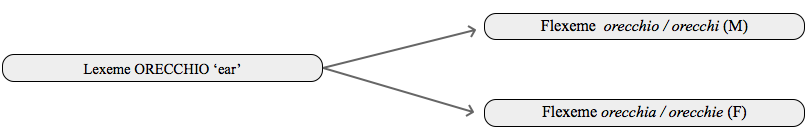
\includegraphics[width=1\textwidth]{figures/ThorntonFig2.png}
\caption{Mapping between one \isi{lexeme} and two flexemes in \ili{Italian}.}
\label{fig:Thornton:2}
\end{figure}
 
The flexemes are distinct; they instantiate nouns of different
inflectional classes, while most \ili{Italian} noun lexemes\is{lexeme} map to only one
flexeme, belonging consistently to only one gender\is{gender} and one inflectional
class, as shown by the examples in Table \ref{tab:Thornton:2}.

  \begin{table}
  \begin{tabular}{llll}
  \lsptoprule
lexeme & \multicolumn{2}{c}{flexeme} & gloss\\
& \textsc{sg} & \textsc{pl} &\\
\midrule
\textsc{occhio (m)} & \emph{occhio} & \emph{occhi} & `eye'\\
\textsc{bocca(f)} & \emph{bocca} & \emph{bocche} & `mouth'\\
\textsc{mano(f)} & \emph{mano} & \emph{mani} & `hand'\\

\lspbottomrule
\end{tabular}
\caption{\ili{Italian} (personal knowledge).}
\label{tab:Thornton:2}
\end{table}

  
Lexemes\is{lexeme} such as \textsc{braccio\textsuperscript{1}, ginocchio} and
\textsc{orecchio} are non-canonical, in that they map to more than one
flexeme, as seen above.

The last case of non-canonical mapping between lexemes\is{lexeme} and flexemes that
I will examine is that of certain \ili{Italian} verbs, that are described as
able to inflect according to two different conjugations; these are
called ``verbi sovrabbondanti'' by %
%Serianni (1988)
\citet{Serianni1988}%
%Serianni
%
.


Grammars usually address together two kinds of such verbs: those in
which the difference in conjugation does not bring along a difference in
meaning (\ref{ex:Thornton:13a}), and those in which the difference in inflectional class
goes hand in hand with a difference in meaning (\ref{ex:Thornton:13b}).

\ea\label{ex:Thornton:13} \ili{Italian} %
(%
%Serianni 1988
\citealt{Serianni1988}%
%
, personal knowledge)
%\citep[, personal knowledge]{Serianni1988}%
%Serianni
%


\ea\label{ex:Thornton:13a}

\ea \emph{adempiere\slash{}adempire} \\
\glt `fulfil'\\

\ex \emph{compiere\slash{}compire} \\
\glt `complete'\\

\ex \emph{empiere\slash{}empire} \\
\glt `fill'\\

\ex \emph{riempiere\slash{}riempire }\\
\glt `fill'\\
\z
\ex\label{ex:Thornton:13b}

\ea \emph{abbonare\slash{}abbonire} \\
\glt `subscribe'\slash{}`appease'\\

\ex \emph{arrossare\slash{}arrossire} \\
\glt `make red', `dye red'\slash{}`redden', `flush'\\

\ex \emph{fallare\slash{}fallire} \\
\glt `make a mistake'\slash{}`fail'\\

\ex \emph{imboscare\slash{}imboschire} \\
\glt `hide {[}in a wood{]}'\slash{}`afforest'\\

\ex \emph{impazzare\slash{}impazzire} \\
\glt `be in full swing'\slash{}`go crazy'\\

\ex \emph{sfiorare\slash{}sfiorire} \\
\glt `brush', `graze'\slash{}`wither', `wilt'\\

\z
\z
\z

%
%Serianni (1988)
\citet{Serianni1988}%
%Serianni
%
, from which the examples in (\ref{ex:Thornton:13}) are taken, considers
the cases in (\ref{ex:Thornton:13}a) and (\ref{ex:Thornton:13}b) as two groups of overabundant\is{overabundance} verbs, while
%
%Dardano \& Trifone (1985) 
\citet{DardanoTrifone1985} %
%Dardano-Trifone
%
consider only cases (\ref{ex:Thornton:13}a) as overabundant\is{overabundance}
verbs, and propose that cases in (\ref{ex:Thornton:13}b) are best analyzed as distinct
lexemes\is{lexeme}; I concur with Dardano \& Trifone, because of a clear difference
in meaning between the two verbs in each pair in (\ref{ex:Thornton:13}b); these verbs are
different lexemes\is{lexeme} according to \citepos{Fradin2003} and \citepos{Fradin03b}
criteria, and will not be further discussed here.

Verbs in (\ref{ex:Thornton:13}a) are claimed to have forms belonging to the two
inflectional classes traditionally called 2\textsuperscript{nd}
conjugation (infinitive ending in -\emph{ere}) and 3\textsuperscript{rd}
conjugation (infinitive ending in -\emph{ire}); besides, the
3\textsuperscript{rd} conjugation forms belong to the subclass of
3\textsuperscript{rd} conjugation verbs which does not exhibit the
element -\emph{isc}- in the appropriate morphomic partition (so
\textsc{prs.ind.1sg} is \emph{empio}, not *\emph{empisco}, etc.). The
2\textsuperscript{nd} conjugation and the -\emph{isc}-less subclass of
the 3\textsuperscript{rd} conjugation have non-distinct inflection in
several cells, listed in (\ref{ex:Thornton:14}a), while they have distinct forms in other
cells, listed in (\ref{ex:Thornton:14}b), with examples from \emph{riempiere} and
\emph{riempire}:\footnote{In (\ref{ex:Thornton:14}) I consider only synthetic forms;
  periphrastic forms are formed by an inflected auxiliary followed by a
  Past Participle\is{verb!past participle}, so their distinctness is a function of the
  distinctness of the Past Participle\is{verb!past participle} form (therefore, they are always
  distinct for these two conjugations).}

\ea\label{ex:Thornton:14} \ili{Italian} (personal knowledge)


\ea\label{ex:Thornton:14a}Cells with non-distinct realization for the verbs in (\ref{ex:Thornton:13}a)

Present Indicative: all person\slash{}number forms, except \textsc{2pl}

Present Subjunctive: all person\slash{}number forms

Imperative \textsc{2sg }

Gerund

(Present Participle)\footnote{A so-called Present Participle ending in
  -\emph{nte} is normally listed as part of a verb's \isi{paradigm} in \ili{Italian}
  descriptive grammars, but it is extremely doubtful that such a cell
  should be recognized as a genuine part of verbal paradigms\is{paradigm} in \ili{Italian}.
  %
%Haspelmath (1996) 
\citet{Haspelmath1996} %
%Haspelmath
%
contrasts these so-called present participles of
  \ili{Italian} with those of other languages in terms of their syntactic
  properties (government of subject and non-subject arguments) and
  concludes that in \ili{Italian} ``active participles do not exist''
  %
%(Haspelmath 1996: 61)
\citep[61]{Haspelmath1996}%
%Haspelmath
%
. %
%Luraghi (1999) 
\citet{Luraghi1999a} %
%Luraghi
%
is less drastic, but shows that
  -\emph{nte} forms have never been part of the spoken register in the
  history of the language, and that a verbal usage of -\emph{nte} forms
  is only attested in some technical or bureaucratic registers, while
  adjectives and nouns in -\emph{nte}, often unrelated to any verbal
  base, are common.}

\ex\label{ex:Thornton:14b}Cells with distinct realization for the verbs in (\ref{ex:Thornton:13}a)

Present Indicative \textsc{2pl =} Imperative \textsc{2pl} (e.g.,
\emph{riempiete} vs. \emph{riempite})

Imperfective Past Indicative (\emph{Imperfetto}): all person\slash{}number
forms (e.g., \textsc{1sg} \emph{riempievo} vs. \emph{riempivo,} etc.)

Simple Perfective Past Indicative (\emph{Passato Remoto}): all
person\slash{}number forms (e.g., \textsc{1sg} \emph{riempietti} or
\emph{riempiei} vs. \emph{riempii,} etc.)

Future: all person\slash{}number forms (e.g., \textsc{1sg} \emph{riempierò} vs.
\emph{riempirò,} etc.)

Imperfect Subjunctive: all person\slash{}number forms (e.g., \textsc{1sg}
\emph{riempiessi} vs. \emph{riempissi,} etc.)

Present Conditional: all person\slash{}number forms (e.g., \textsc{1sg}
\emph{riempierei} vs. \emph{riempirei,} etc.)

Past Participle\is{verb!past participle} (e.g., \emph{riempiuto} vs. \emph{riempito})

Infinitive (e.g., \emph{riempiere} vs. \emph{riempire})

\z
\z

The verbs in (\ref{ex:Thornton:13}a) are technically cases of single lexemes\is{lexeme} mapping to
two distinct flexemes, but these flexemes are syncretic in all the cells
listed in (\ref{ex:Thornton:14}a).

As I am always wary of believing statements by grammars on the
distribution of cell mates\is{cell mate}, I have checked the distribution in the
corpus \emph{la Repubblica 1985-2000} of the forms of the verbs in (\ref{ex:Thornton:13}a)
that are distinct in the two conjugations. Table~\ref{tab:Thornton:3} illustrates the
results (figures for forms of the same Tense\slash{}Mood have been added
together).

\begin{sidewaystable}
\begin{tabular}{lllllllll}
\lsptoprule
& \textsc{empiere} & \textsc{empire} & \textsc{riempiere} &
\textsc{riempire} & \textsc{adempiere} & \textsc{adempire} &
\textsc{compiere} & \textsc{compire}\\
\midrule
\textsc{2pl.prs.ind} = \textsc{2pl.imp} & -\/- & 1 & -\/- & 368 & -\/- &
2 & -\/- & 2\\
\emph{Imperfetto} & -\/- & 2 & 2 & 611 & -\/- & 10 & 7 &
441\\
\emph{Passato Remoto} & 1 & 5 & -\/- & 282 & -\/- & 7 & -\/- &
423\\
Future & 1 & -\/- & -\/- & 294 & 5 & 27 & 23 & 1371\\
Imperfect Subjunctive & -\/- & -\/- & -\/- & 52 & -\/- & 7 & 7 &
111\\
Present Conditional & -\/- & -\/- & -\/- & 52 & -- & 3 & 3 &
76\\
Past Participle & -\/- & -\/- & -\/- & 2307 -\emph{o}& 233 -\emph{o} & -\/- & 15907 -\emph{o} & ? -\emph{o}\\

 &  &  & &
537 -\emph{a} &
10 -\emph{a} &  &
4700 -\emph{a} &
3 -\emph{a}\\

& &  &  &
450 -\emph{i} &
24 -\emph{i} &&
5926 -\emph{i} &

? -\emph{i}\\

 &  & &  &
368 -\emph{e} &
24 -\emph{e} &&
2397 -\emph{e} &

1 -\emph{e}\\

Infinitive & -\/- & 3 & 15 & 3239 & 615 & 4 & 9267 & 8\\
Total & 2 & 11 & 17 & 8560 & 911 & 60 & 38237 & \textgreater{}
2400\\
\lspbottomrule
\end{tabular}
\caption{Frequency in \emph{la Repubblica 1985-2000} corpus of forms of the verbs in (\ref{ex:Thornton:13a}) in cells that have distinct realizations for the two conjugations.}
\label{tab:Thornton:3}
\end{sidewaystable}


The data in Table~\ref{tab:Thornton:3} show the following picture: \textsc{empiere\slash{}empire} `fill' are almost extinct verbs in both conjugations, totaling
only 13 forms overall; their meaning is normally expressed, in
contemporary \ili{Italian}, by \textsc{riempire}; \textsc{riempiere} `fill' is
little used -- there are a few tokens of the Infinitive and of the
Imperfective Past Indicative (\emph{Imperfetto}) in usage, but the ratio
between forms of \textsc{riempire} and forms of \textsc{riempiere} in
the cells for which the two conjugations have distinct forms is so
unbalanced (504:1) that the two verbs represent at best an extremely
weak and non-canonical case of \isi{overabundance} (or mapping from one \isi{lexeme}
to two flexemes) according to %
%Thornton's (2012: 188-189) 
\citeposp{Thornton12}{188--189} %
%Thornton
%
criteria for
measuring the strength of \isi{overabundance} on the basis of frequency ratios
between two cell mates\is{cell mate}. \textsc{Adempiere} and \textsc{adempire}
`fulfil' have a less unbalanced frequency ratio (15.2:1) overall, but it
must be observed that 99.5\% of the forms of \textsc{adempiere} are
realizations of the Infinitive and the Past Participle\is{verb!past participle}, while 93.3\% of
the forms of \textsc{adempire} are realizations of tenses different from
the Infinitive and the Past Participle\is{verb!past participle}. Indeed, all the Past Participle\is{verb!past participle}
forms are 2\textsuperscript{nd} conjugation forms (i.e., they are forms
of \textsc{adempiere}, not possible forms of \textsc{adempire}), so
there is no \isi{overabundance} in this cell; the only tenses in which the two
verbs display some \isi{overabundance} are the Future (with a ratio of 5.4:1
in favour of \textsc{adempire}) and, very marginally, the Infinitive
(with a very unbalanced ratio of 154:1 in favour of \textsc{adempiere}).
The same picture, even more dramatically, is presented by
\textsc{compiere\slash{}compire} `complete'. Assessment of \isi{overabundance} in
this case is made difficult by the fact that some Past Participle\is{verb!past participle} forms
of \textsc{compire} are homographous with other forms in the \isi{paradigm},
and\slash{}or with forms of the noun \textsc{compito} `task, homework', and\slash{}or of the adjective \textsc{compito} `corteous, polite', and\slash{}or of the
verb \textsc{compitare} `spell out' (e.g., \emph{compito} represents
`complete.\textsc{pst.ptcp.m.sg}', `task(\textsc{m}).\textsc{sg}',
`courteous.\textsc{m.sg}' and `spell\_out.\textsc{prs.ind.1sg}'; the
noun for `task' and the \textsc{1sg} form of `spell out' have
antepenultimate stress, while the other forms have penultimate stress,
but stresses on these syllables are not marked in the standard
orthography of \ili{Italian}, so all the forms are homographs even if they are
not all homophonous); these homographies have been manually
disambiguated for the forms ending in -\emph{a} and -\emph{e}
(\emph{compita} `complete.\textsc{pst.ptcp.f.sg}',
`courteous\textsc{.f.sg}', `spell\_out.\textsc{prs.ind.3sg}' and
\emph{compite} `complete.\textsc{pst.ptcp.f.pl}',
`complete.\textsc{prs.ind.2pl}', `courteous\textsc{.f.pl}'), which have
low frequency, thus making manual disambiguation practical; the lack of
manual disambiguation for the high frequency forms in -\emph{o} and
\emph{-i} explains why the exact frequency of these forms is not given
in Table~\ref{tab:Thornton:3}, and a question mark has been inserted instead.\footnote{The
  raw frequency in \emph{la Repubblica} \emph{1985-2000} of the form
  \emph{compito} is 26450, that of \emph{compiti} 9180.} The actual
forms realizing `complete.\textsc{pst.ptcp.f.sg}', and
`complete.\textsc{pst.ptcp.f.pl}' turned out to be a minority (3 over 48
(6\%) for the \textsc{f.sg} form, 1 over 9 (11\%) for the \textsc{f.pl}
form). Therefore, it may be concluded with some safety that in the Past
Participle cell the verb \textsc{compiere} is favoured and
\textsc{compire} is quite underrepresented. These two verbs show the
same kind of ``division of labour'' already observed for
\textsc{adempiere} and \textsc{adempire}: \textsc{compiere} specializes
for the Infinitive and the Past Participle\is{verb!past participle}, and \textsc{compire} for all
other tenses (among the ones that have distinct realizations for the two
conjugations); however, in most tenses a few forms of \textsc{compiere}
are also attested, so \textsc{compiere\slash{}compire} represent the best
example of \isi{overabundance} in all cells encountered so far among the
\ili{Italian} verbs commonly dubbed ``sovrabbondanti'' (although the frequency
ratios render this case of \isi{overabundance} not very canonical). It seems
that \textsc{adempiere\slash{}adempire} and \textsc{compiere\slash{}compire} are
on their way from \isi{overabundance} to \isi{heteroclisis}: at some point in the
future, we might observe a \isi{lexeme} with finite synthetic forms belonging
to the 3\textsuperscript{rd} conjugation and Infinitive and Past
Participle (which carries with it all the periphrastic forms) belonging
to the 2\textsuperscript{nd} conjugation. \textsc{Riempiere\slash{}riempire},
instead, is just reducing \isi{overabundance} in favour of the
3\textsuperscript{rd} conjugation forms, and is quite advanced in this
process.

If the process leading to \isi{heteroclisis} is completed, we will have a
single \isi{lexeme} mapping to a single heteroclitic flexeme. At the moment,
however, we have a number of \ili{Italian} verbal lexemes\is{lexeme} that map to two
flexemes, at least in parts of their \isi{paradigm}.\footnote{A reviewer
  observes that one could introduce \isi{overabundance} in the very make-up of
  flexemes, rather than using it as the grounds for positing two (or
  more) distinct flexemes whenever a \isi{lexeme} has two (or more) distinct
  realizations for a single cell, as done in this paper. This would
  involve allowing flexeme cells to comprise sets of forms rather than a
  single form. The relative merits of the two alternative approaches
  could be fully compared only in a formalized model, whose development
  exceeds the scope of this paper.}

\section{Conclusions}\label{conclusions}

The data illustrated in this paper show that the distinction between
lexemes\is{lexeme} and flexemes first proposed by %
%Fradin \& Kerleroux (2003) 
\citet{Fradin03b} %
%Fradin-Kerleroux
%
and
%
%Fradin (2003)
\citet{Fradin2003}%
%Fradin
%
, as well as their definition of \isi{lexeme} based on semantic
and constructional coherence, is useful even beyond the area of \isi{lexeme}
formation, for which it was originally proposed. A separation between
lexemes\is{lexeme} and flexemes, like the separation between content paradigms\is{paradigm},
form paradigms\is{paradigm!form paradigm} and realized paradigms\is{paradigm!realized paradigm} adopted in paradigm-linkage
theory, is a useful tool in models of morphological analysis that
recognize a level of \is{morphology!autonomous}autonomous morphology.


%\nocite{Acquaviva2008}
%\nocite{Aronoff94}
%\nocite{Aronoff2000b}
%\nocite{BattagliaPernicone1954}
%\nocite{Bonami12t}
%\nocite{Bolinger1956}
%\nocite{chapters/BonamiCrysmann}
%\nocite{Bonami:Stump16:PFM}
%\nocite{ButtBenjamin2013}
%\nocite{Carstairs1987}
%\nocite{Corbett2005}
%\nocite{Corbett2006}
%\nocite{Corbett2007}
%\nocite{DardanoTrifone1985}
%\nocite{Fradin2003}
%%\nocite{Fradin17}
%\nocite{Fradin03b}
%\nocite{Fradin09}
%\nocite{Haspelmath1996}
%\nocite{Holes1995}
%\nocite{Kaye2007}
%\nocite{BaroniBernardiniEtAl2004} % La Repubblica
%\nocite{Luraghi1999a}
%\nocite{RojoVeiga1999}
%\nocite{Serianni1988}
%\nocite{Stump16}
%\nocite{Thornton2011b}
%\nocite{Thornton11}
%\nocite{Thornton12}
%\nocite{Thornton2014}
%\nocite{Thornton2016}
%\nocite{Trepos1994}
%\nocite{Ullmann1957}
%\nocite{Zingarelli2016}

\nocite{laRepubblica}

\is{flexeme|)}


{\sloppy
    \printbibliography[heading=subbibliography,notkeyword=this]
}

\end{document}
